% ===================================================================
%  Week 1 — Lecture Notes (Persian) — Digital Images & the Pipeline
%  Compile: xelatex -interaction=nonstopmode notes.tex   (twice)
% ===================================================================
\documentclass[12pt,a4paper]{article}
% ===================================================================
%  Shared preamble for Persian lecture notes (Image Processing).
%  Compile with XeLaTeX.  Body = Persian (RTL), code/math = LTR.
% ===================================================================

\usepackage{geometry}
\geometry{a4paper,margin=2.4cm}
\usepackage{amsmath,amssymb}
\usepackage{graphicx}
\usepackage{xcolor}
\usepackage{listings}
\usepackage{tcolorbox}
\usepackage{booktabs}
\usepackage{array}
\usepackage{enumitem}
\usepackage{hyperref}
\tcbuselibrary{skins,breakable}

% ---- Persian / RTL --------------------------------------------------
\usepackage{xepersian}
\settextfont{IRNazli}
\setlatintextfont{Latin Modern Roman}
\setdigitfont{IRNazli}
% More generous leading + paragraph spacing (Persian reads better with air).
\linespread{1.5}
\setlength{\parskip}{0.7em}

% ---- Colours --------------------------------------------------------
\definecolor{coursePrimary}{HTML}{1B4965}
\definecolor{courseAccent}{HTML}{E76F51}
\definecolor{courseGood}{HTML}{2A9D8F}
\definecolor{courseBad}{HTML}{C0392B}
\definecolor{courseInfo}{HTML}{2980B9}
\definecolor{codeBg}{HTML}{F5F6FA}
\definecolor{codeKw}{HTML}{8E44AD}
\definecolor{codeStr}{HTML}{2A9D8F}
\definecolor{codeCom}{HTML}{7F8C8D}

\hypersetup{colorlinks=true,linkcolor=courseInfo,urlcolor=courseInfo,citecolor=courseInfo}

% ---- Code listings (Python built in) -------------------------------
\lstdefinestyle{course}{
  backgroundcolor=\color{codeBg},
  basicstyle=\ttfamily\small,
  keywordstyle=\color{codeKw}\bfseries,
  stringstyle=\color{codeStr},
  commentstyle=\color{codeCom}\itshape,
  numberstyle=\tiny\color{codeCom},
  numbers=left, numbersep=7pt,
  showstringspaces=false, breaklines=true,
  tabsize=4, columns=fullflexible, frame=single,
  rulecolor=\color{gray!30}, keepspaces=true, upquote=true, language=Python,
}
\lstset{style=course}
\lstdefinelanguage{bash}{
  keywords={cd,pip,python,venv,source,import}, sensitive=true,
  morecomment=[l]{\#}, morestring=[b]', morestring=[b]",
}
\newenvironment{ltrcode}{\begin{LTR}}{\end{LTR}}

% ---- Callout boxes (Persian titles) --------------------------------
\newtcolorbox{yaddasht}{colback=courseInfo!8,colframe=courseInfo,
  title={\textbf{یادداشت}},boxrule=0.6pt,right=6pt,left=6pt,breakable}
\newtcolorbox{nokte}{colback=courseAccent!10,colframe=courseAccent,
  title={\textbf{نکتهٔ کلیدی}},boxrule=0.6pt,right=6pt,left=6pt,breakable}
\newtcolorbox{hoshdar}{colback=courseBad!8,colframe=courseBad,
  title={\textbf{هشدار / دام}},boxrule=0.6pt,right=6pt,left=6pt,breakable}
\newtcolorbox{riyazi}{colback=coursePrimary!6,colframe=coursePrimary,
  title={\textbf{ریاضیات}},boxrule=0.6pt,right=6pt,left=6pt,breakable}
\newtcolorbox{tamrin}{colback=courseGood!8,colframe=courseGood,
  title={\textbf{تمرین}},boxrule=0.6pt,right=6pt,left=6pt,breakable}

% ---- Header helper --------------------------------------------------
\newcommand{\coursemeta}[2]{%
  \begin{center}
  {\large\textbf{پردازش تصویرِ کاربردی}}\\[2pt]
  {\color{coursePrimary}\rule{\linewidth}{1pt}}\\[4pt]
  {\Large\textbf{#1}}\\[3pt]
  {\small جزوهٔ درس — #2}
  \end{center}\vspace{4pt}
}


\begin{document}
\coursemeta{جلسهٔ ۱ — تصویرِ دیجیتال و خطِ لولهٔ پردازش}{هفتهٔ اول}

{\small\itshape مکملِ اسلایدهای انگلیسیِ جلسهٔ ۱. هدف: فهمِ اینکه یک تصویرِ دیجیتال واقعاً چیست، چطور در کد نمایش داده می‌شود، و کلِ کورس چه مسیری را طی می‌کند.}

\vspace{0.5cm}
\tableofcontents
\vspace{1cm}

% ===================================================================
\section{مقدمه و مقصدِ کورس}

تا پایانِ کورس، شما \textbf{DocScan} را می‌سازید: یک عکس از یک سند (صفحه، فرم، رسید) که با زاویه
و نورِ ناهموار گرفته شده $\rightarrow$ یک اسکنِ تمیز، صاف‌شده و قابلِ‌خواندنِ ماشینی، و سپس خواندنِ
بخشی از محتوا با یک شبکهٔ عصبیِ کوچک. ابزارها: \lr{Python + OpenCV + NumPy}. جلسات ۱ تا ۱۱
پردازشِ تصویرِ کلاسیک، و جلسات ۱۲ تا ۱۴ مقدمهٔ یادگیریِ عمیق برای بینایی.

\begin{nokte}
عادتی که می‌سازیم: \emph{اول} پیکسل‌ها و ریاضی را بفهم؛ \emph{دوم} کتابخانه را صدا بزن؛ و سراغِ
یک شبکهٔ عصبی فقط وقتی برو که روش‌های کلاسیک کم بیاورند. این ترتیب، تفاوتِ کسی که «تابع صدا
می‌زند» و مهندسی که «می‌داند چرا» را می‌سازد.
\end{nokte}

\subsection{چرا پردازش تصویر؟}

پردازش تصویر همه‌جا هست: تشخیصِ پزشکی (تومور در MRI)، خودروی خودران (تشخیصِ خطوط و عابر)،
کنترلِ کیفیتِ صنعتی (تشخیصِ عیب)، امنیت (تشخیصِ چهره)، کشاورزی (سلامتِ محصول از تصویرِ هوایی)،
و اسناد (OCR، همان DocScanِ ما). در همهٔ این‌ها، مسئله یکی است: از پیکسل‌های خام به یک تصمیمِ
معنادار رسیدن. تکنیک‌های این کورس، بلوک‌های سازندهٔ همهٔ این کاربردهاست.

\begin{yaddasht}
پردازش تصویرِ کلاسیک (که تا جلسهٔ ۱۱ می‌آموزیم) هنوز حیاتی است، حتی در عصرِ یادگیریِ عمیق: سریع،
قابلِ‌تفسیر، بدونِ نیاز به دادهٔ آموزشیِ عظیم، و اغلب پیش‌پردازشِ لازم پیش از یک شبکهٔ عصبی. بهترین
سیستم‌ها کلاسیک و عمیق را ترکیب می‌کنند — دقیقاً کاری که DocScan می‌کند.
\end{yaddasht}

\subsection{راه‌اندازیِ محیط}

\begin{ltrcode}
\begin{lstlisting}[language=bash]
python -m venv venv
source venv/bin/activate        # Windows: venv\Scripts\activate
pip install numpy opencv-python scikit-image matplotlib
# deep-learning weeks (12-14):
pip install torch torchvision
\end{lstlisting}
\end{ltrcode}

\lr{NumPy} موتورِ آرایه است؛ \lr{OpenCV} کتابخانهٔ اصلیِ پردازش تصویر؛ \lr{scikit-image} مکملِ
پایتونیک‌تر؛ \lr{Matplotlib} برای نمایش. همه روی نسخه‌های سازگار باشند تا کدها یکسان اجرا شوند.

\subsection{خطِ لولهٔ پردازش تصویر}

تقریباً هر تسک در این کورس مسیری در این خطِ لوله است:
\[
\text{اکتساب} \rightarrow \text{پیش‌پردازش} \rightarrow \text{بهبود} \rightarrow \text{قطعه‌بندی}
\rightarrow \text{استخراجِ ویژگی} \rightarrow \text{تصمیم}
\]
DocScan همهٔ این مسیر را می‌پیماید: از عکسِ خام تا خواندنِ محتوا.

% ===================================================================
\section{تصویرِ دیجیتال چیست؟}

\subsection{تصویر، یک تابعِ نمونه‌برداری‌شده روی یک شبکه است}

یک تصویرِ پیوسته یک تابعِ $f(x,y)$ است: روشناییِ نقطه‌ای در موقعیتِ $(x,y)$. یک تصویرِ
\textbf{دیجیتال} این تابع را روی یک شبکه \emph{نمونه‌برداری} می‌کند و هر مقدار را \emph{گِرد}
می‌کند؛ نتیجه \textbf{پیکسل}‌ها هستند. یک تصویرِ خاکستری یک آرایهٔ دوبعدی است؛ یک تصویرِ رنگی سه
آرایهٔ این‌چنینی (کانال).

\begin{riyazi}
$f(x,y)$ با $x = 0,\dots,W{-}1$ و $y = 0,\dots,H{-}1$، و هر مقدار در مجموعهٔ
$\{0,\dots,255\}$ (برای ۸ بیت). صفر = سیاه، ۲۵۵ = سفید، بینابین = خاکستری.
\end{riyazi}

\subsection{یک تصویرِ واقعی از دیتاست}

مثالِ در‌جریانِ ما یک نمای شمارندهٔ کنتورِ آب است (از دیتاستِ شما،
\lr{E:/data/abfa\_image/numerators}). خواندنِ همین ارقام، دقیقاً هدفِ پروژهٔ نهاییِ DocScan است.

\begin{center}
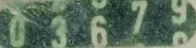
\includegraphics[width=0.7\linewidth]{../assets/meter_bgr.png}\\[2pt]
{\small تصویرِ اصلیِ رنگی — یک نمای رقمِ کنتور ($48\times196$ پیکسل)}\\[6pt]

\includegraphics[width=0.7\linewidth]{../assets/meter_gray.png}\\[2pt]
{\small نسخهٔ خاکستری — یک کانال، همان ساختار}
\end{center}

\subsection{پیکسل‌ها فقط عددند}

«پردازشِ» یک تصویر یعنی انجامِ محاسبات روی این اعداد. هیچ جادویی وجود ندارد: هر عملیات،
ریاضی روی یک آرایه است. این جملهٔ ساده، کلِ فلسفهٔ کورس است — وقتی یک فیلتر، یک آستانه، یا یک
تشخیصِ لبه را می‌بینید، در پسِ آن فقط جمع، ضرب، و مقایسهٔ اعداد است.

\subsection{نمونه‌برداری: چه‌قدر دقیق مکان را می‌سنجیم}

\textbf{نمونه‌برداری} (\lr{sampling}) = انتخابِ نقاطِ شبکه (وضوح، \lr{resolution}). نمونه‌های
خیلی کم یعنی از‌دست‌رفتنِ جزئیات — یا بدتر، جعلِ آن (\lr{aliasing}، در بخشِ عمیق). پیکسل‌های
بیشتر = جزئیاتِ مکانیِ بیشتر و دادهٔ بیشتر.

\subsection{کوانتش: چه‌قدر دقیق روشنایی را می‌سنجیم}

\textbf{کوانتش} (\lr{quantization}) = گِردکردنِ هر نمونه به مجموعهٔ متناهی از سطوح (عمقِ بیت،
\lr{bit depth}). ۸ بیت = ۲۵۶ سطح (۰ تا ۲۵۵)؛ ۱ بیت = سیاه/سفید؛ ۱۶ بیت = ۶۵۵۳۶ سطح
(پزشکی/\lr{RAW}). سطوحِ خیلی کم $\rightarrow$ \textbf{نوارنوارشدنِ} (\lr{banding}) دیدنی در
گرادیان‌های نرم.

\begin{yaddasht}
وضوح (نمونه‌برداری) و عمقِ بیت (کوانتش) دو محورِ «چه‌قدر تصویر داریم» هستند: یکی دقتِ مکانی،
دیگری دقتِ روشنایی. هر دو حجمِ داده و کیفیت را تعیین می‌کنند.
\end{yaddasht}

\subsection{وضوح، اندازه، و حافظه}

یک تصویرِ خاکستریِ ۸ بیتیِ $W\times H$ برابرِ $W\cdot H$ بایت است؛ رنگی سه برابر. یک عکسِ
رنگیِ ۱۲ مگاپیکسلی حدودِ ۳۶ مگابایت \emph{فشرده‌نشده} است. برای همین فرمت‌ها فشرده می‌کنند — و
برای همین پردازشِ تصاویرِ بزرگ به دقت نیاز دارد (جلسهٔ ۱۱). پیش از هر کاری شکل و نوعِ دادهٔ تصویر
را بدانید: \lr{img.shape} و \lr{img.dtype}.

% ===================================================================
\section{رنگ}

\subsection{رنگ: سه عدد به‌ازای هر پیکسل}

\textbf{RGB}: کانال‌های قرمز، سبز، آبی؛ همان‌طور که نمایشگرها نور می‌تابانند. یک پیکسلِ رنگی یک
سه‌تایی $(R,G,B)$ است، هرکدام ۰ تا ۲۵۵. خاکستری‌سازی رنگ را به یک روشنایی فرومی‌کاهد — اغلب اولین
گام (دادهٔ کمتر، ساختارِ یکسان).

\begin{riyazi}
روشنایی (\lr{luminance}): $Y = 0.299R + 0.587G + 0.114B$. سبز غالب است چون چشمِ ما به سبز
حساس‌تر است. این وزن‌دهیِ ادراکی، از میانگینِ سادهٔ $(R+G+B)/3$ درست‌تر است.
\end{riyazi}

\subsection{چرا به خاکستری تبدیل کنیم}

بسیاری از عملیات (لبه، آستانه) به روشنایی نیاز دارند، نه رنگ — یک کانال، یک‌سومِ کار. DocScan
عمدتاً در خاکستری کار می‌کند؛ رنگ فقط وقتی برمی‌گردد که اطلاعات حمل کند. اما خاکستری‌سازی اطلاعات
را \emph{دور می‌ریزد} — اگر رنگ مهم است (مثلاً قطعه‌بندیِ رنگیِ جلسهٔ ۸) این کار را نکنید.

\subsection{فضاهای رنگیِ دیگر و چرایی}

\begin{center}
\begin{tabular}{>{\raggedright\arraybackslash}p{0.18\linewidth} >{\raggedright\arraybackslash}p{0.3\linewidth} >{\raggedright\arraybackslash}p{0.42\linewidth}}
\toprule
\textbf{فضا} & \textbf{کانال‌ها} & \textbf{مناسبِ} \\
\midrule
\lr{RGB} & قرمز، سبز، آبی & ذخیره، نمایش \\
خاکستری & روشنایی & بیشترِ پردازشِ کلاسیک \\
\lr{HSV} & رنگ‌مایه، اشباع، مقدار & انتخابِ رنگ‌محور (مقاوم به نور) \\
\lr{Lab} & روشنایی، a، b & فاصلهٔ ادراکی، تصحیحِ رنگ \\
\bottomrule
\end{tabular}
\end{center}

\begin{nokte}
انتخابِ فضای رنگیِ درست می‌تواند یک مسئلهٔ سخت را آسان کند — مثلاً «شیءِ قرمز را پیدا کن» در
\lr{HSV} بدیهی است و در \lr{RGB} دردناک. در \lr{HSV}، رنگ‌مایه (\lr{Hue}) رنگ را از روشنایی جدا
می‌کند، پس انتخاب در برابرِ سایه و نور مقاوم می‌شود.
\end{nokte}

% ===================================================================
\section{تصاویر در کد}

\subsection{تصویر یک آرایهٔ NumPy است}

\begin{ltrcode}
\begin{lstlisting}[language=Python]
import cv2, numpy as np
img = cv2.imread('page.jpg')          # BGR, shape (H, W, 3), dtype uint8
print(img.shape, img.dtype)           # e.g. (1200, 900, 3) uint8
gray = cv2.cvtColor(img, cv2.COLOR_BGR2GRAY)  # (H, W)
print(gray[0, 0])                     # a single pixel's intensity, 0..255
\end{lstlisting}
\end{ltrcode}

\begin{hoshdar}
دامِ OpenCV: تصاویر را به‌صورتِ \textbf{BGR} می‌خواند، نه \lr{RGB}. فراموش‌کردنِ این، قرمز و آبی
را در همه‌جا جابه‌جا می‌کند. پیش از \lr{plt.imshow} حتماً \lr{BGR2RGB} کنید.
\end{hoshdar}

\subsection{پیکسل، برش، و عملیاتِ برداری}

\begin{ltrcode}
\begin{lstlisting}[language=Python]
h, w = gray.shape
roi = gray[100:200, 50:150]           # a rectangular region (a view)
gray[gray < 50] = 0                    # vectorized: dark pixels -> black
brighter = np.clip(gray.astype(int) + 40, 0, 255).astype(np.uint8)
\end{lstlisting}
\end{ltrcode}

\begin{hoshdar}
هرگز در پایتون روی پیکسل‌ها حلقه نزنید — صد برابر کندتر است. از برداری‌سازیِ \lr{NumPy} یا خودِ
\lr{OpenCV} استفاده کنید. این یکی از مهم‌ترین عادت‌های پردازشِ تصویرِ کارآمد است.
\end{hoshdar}

\subsection{نمایش و اشکال‌زداییِ تصویر}

پردازش تصویر بصری است؛ همیشه نتیجهٔ هر گام را ببینید. ابزارها:

\begin{ltrcode}
\begin{lstlisting}[language=Python]
import matplotlib.pyplot as plt
plt.imshow(cv2.cvtColor(img, cv2.COLOR_BGR2RGB)); plt.axis('off'); plt.show()
plt.imshow(gray, cmap='gray', vmin=0, vmax=255)   # grayscale: set the range!
cv2.imwrite('gray.png', gray)                      # PNG = lossless
\end{lstlisting}
\end{ltrcode}

نکتهٔ ظریف: هنگامِ نمایشِ خاکستری با \lr{Matplotlib}، اگر \lr{vmin/vmax} را تنظیم نکنید،
مقادیر به‌طورِ خودکار کشیده می‌شوند و ممکن است تصویری کم‌کنتراست را پرکنتراست \emph{نشان} دهد در
حالی که داده تغییر نکرده. برای دیدنِ واقعیتِ داده، بازه را صریح ۰ تا ۲۵۵ بگذارید. این تفاوتِ
«چیزی که می‌بینید» و «داده‌ای که دارید» یک منبعِ رایجِ سردرگمی است.

\begin{yaddasht}
عادتِ خوب: پس از هر عملیات، \lr{img.min()}، \lr{img.max()}، و \lr{img.dtype} را چاپ کنید. اگر
یک تصویر که باید ۰ تا ۲۵۵ باشد ناگهان ۰ تا ۱ یا اعشاری شد، یک خطا رخ داده. این چند خطِ اشکال‌زدایی
ساعت‌ها گیجی را صرفه‌جویی می‌کند.
\end{yaddasht}

\subsection{دامِ سرریزِ uint8}

محاسبات روی \lr{uint8} \textbf{دور می‌زند} (\lr{wrap around}): $200 + 100 = 44$، نه ۲۵۵! به
\lr{int}/\lr{float} تبدیل کنید، محاسبه کنید، به ۰ تا ۲۵۵ \lr{clip} کنید، و برگردانید. یا از
عملیاتِ اشباعیِ OpenCV (\lr{cv2.add}) که برایتان محدود می‌کند استفاده کنید.

\begin{nokte}
یک «روشن‌سازی» که نواحیِ روشن را تاریک می‌کند، تقریباً همیشه سرریزِ \lr{uint8} است. این یکی از
اولین باگ‌هایی است که هر تازه‌کاری تجربه می‌کند.
\end{nokte}

روی همان تصویرِ کنتور، تفاوت را ببینید:

\begin{center}

\includegraphics[width=0.62\linewidth]{../assets/meter_bright_ok.png}\\[2pt]
{\small \lr{+60} درست (با \lr{clip}): یکنواخت روشن‌تر}\\[6pt]
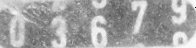
\includegraphics[width=0.62\linewidth]{../assets/meter_bright_overflow.png}\\[2pt]
{\small \lr{+60} در \lr{uint8}: پیکسل‌های روشن \emph{دور زدند} و تاریک شدند}
\end{center}

% ===================================================================
\section{یک مثالِ عددیِ کامل: خاکستری‌سازی}

بیایید تبدیلِ یک پیکسلِ رنگی به خاکستری را دستی انجام دهیم تا فرمول ملموس شود. فرض کنید پیکسلی
داریم با $(R,G,B) = (100, 200, 50)$ (یک سبزِ روشن).

\textbf{میانگینِ ساده:} $(100 + 200 + 50)/3 = 116.67 \approx 117$.

\textbf{روشناییِ ادراکی:} $Y = 0.299(100) + 0.587(200) + 0.114(50) = 29.9 + 117.4 + 5.7 = 153$.

تفاوت چشمگیر است: میانگینِ ساده ۱۱۷ می‌دهد، اما فرمولِ ادراکی ۱۵۳ — چون سبز (که در این پیکسل
غالب است) در ادراکِ انسان وزنِ بیشتری دارد. برای همین یک شیءِ سبز با میانگینِ ساده تیره‌تر از
آنچه باید به‌نظر می‌رسد.

\begin{nokte}
این تفاوت در عمل مهم است: اگر بعداً روی تصویرِ خاکستری آستانه بگذارید (جلسهٔ ۸)، انتخابِ فرمولِ
خاکستری‌سازی می‌تواند نتیجه را عوض کند. کتابخانه‌ها (OpenCV) فرمولِ ادراکی را استفاده می‌کنند؛
بدانید چرا.
\end{nokte}

\subsection{وضوح، DPI، و معنای عملی}

وضوح فقط «تعدادِ پیکسل» نیست؛ نسبتِ آن به اندازهٔ فیزیکی هم مهم است. \textbf{DPI} (نقطه در اینچ)
می‌گوید چند پیکسل به‌ازای هر اینچ داریم. برای DocScan این حیاتی است: یک سند که با DPIِ پایین
اسکن شود، متنِ ریز را از دست می‌دهد و OCR شکست می‌خورد. قاعدهٔ عملی: برای خواندنِ متن، حداقل
۳۰۰ DPI. یک عکسِ موبایلی از فاصلهٔ زیاد ممکن است پیکسل‌های کافی روی هر حرف نداشته باشد — که یکی
از سخت‌ترین چالش‌های پروژهٔ شماست.

% ===================================================================
\section{عملیاتِ حسابیِ تصویر — پیش‌درآمد}

بسیاری از پردازش‌ها ترکیبی از عملیاتِ حسابیِ ساده روی آرایه‌ها هستند:

\begin{itemize}
  \item \textbf{جمع/تفریق}: روشن/تاریک‌کردن، یا تفاوتِ دو تصویر (تشخیصِ تغییر، حذفِ پس‌زمینه).
  \item \textbf{ضرب}: اعمالِ یک ماسک، یا تنظیمِ کنتراست.
  \item \textbf{ترکیب} (\lr{blend}): $\alpha \cdot A + (1-\alpha) \cdot B$ برای محوِ تدریجیِ دو تصویر.
\end{itemize}

مثالِ کاربردی: تفریقِ دو فریمِ متوالیِ یک دوربینِ ثابت، پیکسل‌هایی را که تغییر کرده‌اند (حرکت)
برجسته می‌کند — پایهٔ تشخیصِ حرکت. همهٔ این‌ها فقط جمع و ضربِ آرایه‌اند، با مراقبت از سرریز.

\begin{ltrcode}
\begin{lstlisting}[language=Python]
diff = cv2.absdiff(frame1, frame2)     # |frame1 - frame2|, saturating
blended = cv2.addWeighted(a, 0.7, b, 0.3, 0)  # 0.7*a + 0.3*b
\end{lstlisting}
\end{ltrcode}

% ===================================================================
\section{تمرینِ کلاسیِ وسط‌جلسه (۱۰ دقیقه)}

\begin{tamrin}
پیش‌بینی کنید، بعد اجرا کنید:

\begin{ltrcode}
\begin{lstlisting}[language=Python]
gray = np.array([[100, 150],[200, 250]], dtype=np.uint8)
a = gray + 60          # (1) what are the four values?
b = cv2.add(gray, 60)  # (2) and here?
c = gray.mean()        # (3) what does this represent?
\end{lstlisting}
\end{ltrcode}

(۱) \lr{a} را دستی حساب کنید — مراقبِ سرریز. (۲) \lr{b} چه فرقی دارد؟ (۳) \lr{c} چیست، و یک
\lr{c}ِ خیلی پایین چه چیزی دربارهٔ تصویر می‌گوید؟
\end{tamrin}

\textbf{جمع‌بندی:} \lr{a = [[160,210],[4,54]]} — $200{+}60$ و $250{+}60$ \emph{دور زدند} (سرریز).
\lr{b = [[160,210],[255,255]]} — \lr{cv2.add} اشباع می‌کند (به ۲۵۵ محدود). \lr{c} میانگینِ
روشنایی است ($\approx 175$)؛ میانگینِ خیلی پایین یعنی تصویرِ عمدتاً تاریک (کم‌نور). میانگین/هیستوگرامِ
یک تصویر پیش از نگاه‌کردن، دربارهٔ نوردهی به شما می‌گوید — جلسهٔ ۲.

% ===================================================================
\section{فرمت‌ها و ذخیره‌سازی}

\begin{center}
\begin{tabular}{>{\raggedright\arraybackslash}p{0.16\linewidth} >{\raggedright\arraybackslash}p{0.28\linewidth} >{\raggedright\arraybackslash}p{0.46\linewidth}}
\toprule
\textbf{فرمت} & \textbf{فشرده‌سازی} & \textbf{کاربرد} \\
\midrule
\lr{PNG} & بی‌اتلاف & ماسک، خطوط، نتایجِ میانی \\
\lr{JPEG} & بااتلاف & عکس؛ فایلِ کوچک ولی مصنوعات \\
\lr{TIFF} & بی‌اتلاف/بدون & بایگانی، علمی، چندصفحه \\
\lr{BMP/RAW} & بدون & سادگی / دادهٔ حسگر \\
\bottomrule
\end{tabular}
\end{center}

\begin{hoshdar}
هرگز نتایجِ میانی را \lr{JPEG} ذخیره نکنید — مصنوعاتش پردازشِ بعدی را خراب می‌کنند. \lr{JPEG}
جزئیاتِ فرکانس‌بالا را در بلوک‌های $8\times8$ دور می‌ریزد؛ نامرئی برای چشم، سم برای تشخیصِ لبه.
تا آخرین مرحله \lr{PNG} استفاده کنید. ذخیرهٔ مکررِ یک \lr{JPEG} آسیب را انباشته می‌کند.
\end{hoshdar}

\subsection{عمقِ بیت و بازهٔ دینامیکی}

۸ بیت برای نمایش خوب است؛ حسگرهای ۱۲ تا ۱۶ بیتی جزئیاتِ سایه/های‌لایت را نگه می‌دارند.
\textbf{بازهٔ دینامیکی} = نسبتِ روشن‌ترین به تاریک‌ترین که حسگر می‌تواند ثبت کند. \lr{HDR} چند
نوردهی را ترکیب می‌کند تا از بازهٔ یک حسگر فراتر رود.

% ===================================================================
\section{بخشِ عمیق: مدلِ تصویربرداری}

\subsection{نظریهٔ نمونه‌برداری و آلیاسینگ}

\textbf{نایکوئیست} (\lr{Nyquist}): برای ثبتِ جزئیات در فرکانسِ $f$، با نرخِ بیش از $2f$
نمونه‌برداری کنید. اگر کمتر نمونه بگیرید، فرکانس‌های بالا خود را به‌جای فرکانس‌های پایین جا می‌زنند.
این \textbf{آلیاسینگ} است: الگوهای مواره (\lr{moir\'e})، لبه‌های دندانه‌دار، چرخِ گاری که به عقب
می‌چرخد. راه‌حل: پیش از کاهشِ اندازه، تصویر را تار (پایین‌گذر) کنید — جزئیاتی را که نمی‌توانید
نمایش دهید حذف کنید (جلسات ۳ و ۶).

\begin{hoshdar}
کوچک‌کردنِ یک تصویر بدونِ تارکردنِ اول، مصنوعاتِ آلیاسینگ می‌سازد که هیچ گامِ بعدی نمی‌تواند
جبرانشان کند. این یک اشتباهِ رایج و برگشت‌ناپذیر است.
\end{hoshdar}

\subsection{گاما: پیکسل‌ها نورِ خطی نیستند}

نمایشگرها و فایل‌ها \textbf{گاما-کدشده}‌اند: مقدارِ پیکسل $\ne$ شدتِ نورِ خطی. ذخیرهٔ ادراکی
(کدهای بیشتر برای تُن‌های تاریک، جایی که چشم حساس‌تر است) بیت صرفه‌جویی می‌کند. برای ریاضیِ
\emph{درست} (میانگین‌گیری، ترکیب)، گاهی اول باید خطی‌سازی کنید — یک باگِ ظریفِ رایج.

\begin{riyazi}
کدشده $\approx$ (خطی)$^{1/\gamma}$ با $\gamma \approx 2.2$. از گاما در جلسهٔ ۲ برای کنترلِ
کنتراست استفاده می‌کنیم.
\end{riyazi}

\subsection{پیکسل‌ها از کجا می‌آیند}

\[
\text{صحنه} \rightarrow \text{لنز} \rightarrow \text{حسگر + بایر} \rightarrow \text{دی‌موزائیک + ISP} \rightarrow \text{فایل}
\]
حسگرهای واقعی یک رنگ به‌ازای هر پیکسل ثبت می‌کنند (موزائیکِ \textbf{بایر}، \lr{Bayer}) و بقیه را
درون‌یابی می‌کنند. نویز، تاری، و انحرافِ رنگ اینجا وارد می‌شوند — دقیقاً همان چیزی که پاک‌سازی
می‌کنیم (جلسات ۴ و ۲).

\subsection{نویز فیزیکی است، نه باگ}

شمارشِ فوتون تصادفی است $\rightarrow$ نویزِ شات (\lr{shot noise})؛ الکترونیک نویزِ خواندن اضافه
می‌کند. نورِ کم / \lr{ISO}ی بالا = نویزِ بیشتر. این مادهٔ خامی است که جلسهٔ ۴ حذفش می‌کند. فهمِ
\emph{اینکه} نویز از کجا می‌آید به شما می‌گوید \emph{چطور} مدل و حذفش کنید.

\subsection{صفحاتِ بیتی (Bit planes)}

یک تصویرِ ۸ بیتی را می‌توان به ۸ «صفحهٔ بیتی» تجزیه کرد: صفحهٔ بیتِ ۷ (پرارزش‌ترین) ساختارِ
اصلیِ تصویر را دارد، و صفحهٔ بیتِ ۰ (کم‌ارزش‌ترین) عمدتاً نویز است. این توضیح می‌دهد چرا حذفِ
چند بیتِ کم‌ارزش (کوانتشِ درشت‌تر) تصویر را چندان خراب نمی‌کند اما فضا صرفه‌جویی می‌کند — ایده‌ای
که پشتِ فشرده‌سازی است. همچنین پایهٔ برخی تکنیک‌های پنهان‌نگاری (\lr{steganography}) است که داده
را در بیت‌های کم‌ارزش مخفی می‌کنند.

\subsection{هیستوگرام — نگاهی اجمالی (پیش‌درآمدِ جلسهٔ ۲)}

\textbf{هیستوگرام} یک تصویر می‌شمارد چند پیکسل هر سطحِ روشنایی را دارند. بدونِ نگاه‌کردن به
تصویر، هیستوگرام به شما می‌گوید: آیا تصویر تاریک است (پیک در چپ)، روشن است (پیک در راست)،
کم‌کنتراست است (فشرده در وسط)، یا خوش‌کنتراست (پخش‌شده). این اولین ابزارِ تشخیصیِ شماست و جلسهٔ ۲
کاملاً به آن می‌پردازد. همین حالا بدانید: میانگین و هیستوگرام، «امضای» یک تصویرند.

\subsection{مختصات و قراردادها}

تصاویر با \lr{[row, col] = [y, x]} اندیس‌گذاری می‌شوند — \emph{عکسِ} $(x,y)$ ریاضی. مبدأ
گوشهٔ بالا-چپ است؛ $y$ به \emph{پایین} افزایش می‌یابد. نقاطِ \lr{OpenCV} به‌صورتِ \lr{(x, y)}‌اند
اما اندیس‌های \lr{NumPy} به‌صورتِ \lr{[y, x]}. این‌ها را جدا نگه دارید.

\begin{hoshdar}
جابه‌جاییِ x و y باگِ شمارهٔ یکِ تازه‌کارها در کدِ تصویر است. وقتی چیزی ترانهاده به‌نظر می‌رسد،
اول این را بررسی کنید.
\end{hoshdar}

% ===================================================================
\section{جمع‌بندی}

\begin{itemize}
  \item توضیحِ نمونه‌برداری، کوانتش، وضوح، و عمقِ بیت.
  \item بارگذاریِ تصویر، بازبینیِ شکل/نوع، تبدیلِ رنگ، برشِ نواحی — به‌صورتِ برداری.
  \item انتخابِ فضای رنگی و فرمت برای یک تسک؛ پرهیز از دام‌های \lr{uint8}/\lr{BGR}/\lr{xy}.
  \item نام‌بردنِ منشأِ فیزیکیِ نویز، تاری، و آلیاسینگ.
\end{itemize}

\begin{tamrin}
\textbf{تحویلیِ این هفته (پیش از جلسهٔ ۲):} (۱) سه تصویر را بارگذاری کنید؛ شکل، نوع،
کمینه/بیشینه/میانگین را چاپ کنید؛ به خاکستری و \lr{HSV} تبدیل کنید. (۲) یک \lr{brighten(img, k)}ِ
درست (بدونِ سرریز) بنویسید و با \lr{cv2.add} مقایسه کنید. (۳) یک عکس از یک سند با موبایل بگیرید —
تصویرِ آزمونِ DocScanِ شما. ویژگی‌هایش را گزارش دهید. (۴) یادداشتِ کوتاه: برای عکسِ شما، کدام
گام‌های خطِ لوله سخت‌ترند و چرا؟
\end{tamrin}

\subsection*{چک‌لیستِ دام‌های رایجِ این هفته}

\begin{center}
\begin{tabular}{>{\raggedright\arraybackslash}p{0.42\linewidth} >{\raggedright\arraybackslash}p{0.48\linewidth}}
\toprule
\textbf{دام} & \textbf{راه‌حل} \\
\midrule
BGR در برابرِ RGB & پیش از \lr{imshow}، \lr{cv2.COLOR\_BGR2RGB} \\
سرریزِ \lr{uint8} & به \lr{int} تبدیل، \lr{clip}، برگرداندن؛ یا \lr{cv2.add} \\
جابه‌جاییِ \lr{x} و \lr{y} & اندیسِ \lr{NumPy} برابرِ \lr{[y, x]} است \\
حلقه روی پیکسل‌ها & برداری‌سازیِ \lr{NumPy} \\
ذخیرهٔ میانی به \lr{JPEG} & \lr{PNG} تا آخرین مرحله \\
میانگینِ سادهٔ رنگ & فرمولِ روشناییِ وزن‌دار \\
\bottomrule
\end{tabular}
\end{center}

\subsection*{واژه‌نامهٔ کوتاه}

\begin{center}
\begin{tabular}{>{\raggedright\arraybackslash}p{0.3\linewidth} >{\raggedright\arraybackslash}p{0.6\linewidth}}
\toprule
\textbf{اصطلاح} & \textbf{معنی} \\
\midrule
\lr{Pixel} & کوچک‌ترین عنصرِ تصویر؛ یک مقدارِ روشنایی/رنگ \\
\lr{Sampling} & نمونه‌برداریِ مکانی (وضوح) \\
\lr{Quantization} & گِردکردنِ روشنایی به سطوحِ متناهی (عمقِ بیت) \\
\lr{Channel} & یکی از آرایه‌های رنگ (مثلاً R، G، B) \\
\lr{Aliasing} & جعلِ فرکانس‌بالا در اثرِ کم‌نمونه‌برداری \\
\lr{uint8} & نوعِ ۸ بیتیِ بدونِ‌علامت (۰ تا ۲۵۵)؛ مراقبِ سرریز \\
\bottomrule
\end{tabular}
\end{center}

\vspace{0.5cm}
\begin{center}
\textit{یک تصویر فقط اعدادی روی یک شبکه است. باقیِ کورس، حساب‌وکتاب روی همان اعداد است.}
\end{center}

\end{document}
